\let\negmedspace\undefined
\let\negthickspace\undefined
\documentclass[journal]{IEEEtran}
\usepackage[a5paper, margin=10mm, onecolumn]{geometry}
\usepackage{lmodern} % Ensure lmodern is loaded for pdflatex
 % Include tfrupee package
\setlength{\headheight}{1cm} % Set the height of the header box
\setlength{\headsep}{0mm}     % Set the distance between the header box and the top of the text
\usepackage{enumitem}
\usepackage{gvv-book}
\usepackage{gvv}
\usepackage{cite}
\usepackage{amsmath,amssymb,amsfonts,amsthm}
\usepackage{algorithmic}
\usepackage{graphicx}
\usepackage{textcomp}
\usepackage{xcolor}
\usepackage{txfonts}
\usepackage{listings}
\usepackage{enumitem}
\usepackage{mathtools}
\usepackage{gensymb}
\usepackage{comment}
\usepackage[breaklinks=true]{hyperref}
\usepackage{tkz-euclide} 
\usepackage{listings}
% \usepackage{gvv}                                        
\def\inputGnumericTable{}                                 
\usepackage[latin1]{inputenc}                                
\usepackage{color}                                            
\usepackage{array}                                            
\usepackage{longtable}                                       
\usepackage{calc}                                             
\usepackage{multirow}                                         
\usepackage{hhline}                                           
\usepackage{ifthen}                                           
\usepackage{lscape}
\begin{document}

\bibliographystyle{IEEEtran}
\vspace{3cm}

\title{1-1.2-18}
\author{AI24BTECH11008- Sarvajith
}
% \maketitle
% \newpage
% \bigskip
{\let\newpage\relax\maketitle}

\renewcommand{\thefigure}{\theenumi}
\renewcommand{\thetable}{\theenumi}
\setlength{\intextsep}{10pt} % Space between text and floats
\numberwithin{equation}{enumi}
\numberwithin{figure}{enumi}
\renewcommand{\thetable}{\theenumi}
\textbf{Question: }\\
If the origin is the centroid of the triangle PQR with vertices\\
\textbf{P}\myvec{2a\\2\\ 6} \\ \textbf{Q}\myvec{-4\\3b\\ -10} \\ \textbf{R}\myvec{8\\ 14\\ 2c}\\ then find the values of a, b and
c.\\
\textbf{Solution: }\\
\renewcommand{\tablename}{TABLE 1}
\begin{table}[h!]    
  \centering
  \begin{tabular}{|c|c|}
\hline
\textbf{lengths} & \textbf{values}\\
\hline
\textbf{BC} & 5.5cm\\
\hline
\textbf{AL} & 5.3cm\\
\hline
\end{tabular}

  \caption{values of the geometrical points in given question}
  \label{tab1-1.2-18-1}
\end{table}
\textbf{proof: }\\


\section*{Proof of the Centroid Formula using Matrix Notation}

 Triangle with vertices A\myvec{x_1\\ y_1\\z_1}, B\myvec{x_2\\ y_2\\z_2}, and C\myvec{x_3\\y_3\\z_3}, the centroid G\myvec{x_g\\ y_g\\z_g} 
\begin{align}
The centroid G\myvec{x_g\\y_g\\z_g } can be represented as a column vector:
\begin{align*}
\mathbf{G} = \myvec{ x_g \\ y_g \\ z_g}
\end{align*}

The centroid \brak{G} is the average of the coordinates of the vertices \brak{A} , \brak{B} , and \brak{C}:

\begin{align*}
	\mathbf{G} = \frac{1}{3} \brak{\mathbf{A} + \mathbf{B} + \mathbf{C}}
\end{align*}
 Matrix Addition and Scalar Multiplication
	First, add the vectors \brak{ \mathbf{A} }, \brak{ \mathbf{B} }, and \brak{ \mathbf{C} }:
\begin{align*}
\mathbf{A} + \mathbf{B} + \mathbf{C} = \myvec{ x_1 \\ y_1 \\z_1} + \myvec{ x_2 \\ y_2 \\z_2 } + \myvec{x_3 \\ y_3 \\z_3} = \myvec{ x_1 + x_2 + x_3 \\ y_1 + y_2 + y_3 \\z_1 + z_2 +z_3}
\end{align*}
	Next, multiply by the scalar \brak{ \frac{1}{3} }:
\begin{align*}
	\mathbf{G} = \frac{1}{3} \myvec{ x_1 + x_2 + x_3 \\ y_1 + y_2 + y_3\\z_1+z_2+z_3 } = \myvec {\frac{x_1 + x_2 + x_3}{3} \\ \frac{y_1 + y_2 + y_3}{3} \\ \frac{z_1+z_2+z_3 }{3} }
\end{align*}
\subsection*{Conclusion}
Thus, the coordinates of the centroid G\brak{x_g, y_g,z_g} are given by:
\begin{align*}
    x_g = \frac{x_1 + x_2 + x_3}{3}, \quad y_g = \frac{y_1 + y_2 + y_3}{3}, \quad z_g= \frac{z_1+z_2+z_3}{3}
\end{align*}



This proves the centroid formula using matrix notation.
\begin{equation}
	\textbf{P}\myvec{x_1\\y_1\\z_1} = \myvec{2a\\4\\6}\label{eq1.12.18.1}
\end{equation}
\begin{equation}
    \textbf{Q}\myvec{x_2\\y_2\\z_2} = \myvec{-4\\3\\10}\label{eq1.12.18.2}
\end{equation}
\begin{equation}
    \textbf{R}\myvec{x_3\\y_3\\z_3} = \myvec{8\\14\\2c}\label{eq1.12.18.3}\\
\end{equation}

	Given that, the centroid of the triangle \textbf{PQR} is origin\myvec{0,0,0}. \\
Centroid\brak{G}.\\
From the proof
\begin{align*}
	\mathbf{G} = \frac{1}{3} \brak{\mathbf{P} + \mathbf{Q} + \mathbf{R}}
\end{align*}
	$$G = \brak{\myvec{2a\\4\\6} + \myvec{-4\\3\\10} + \myvec{8\\14\\2c}}\frac{1}{3}$$
        $$G = \myvec{2a-4+8\\4+3+14\\6+10+2c}\frac{1}{3}$$
$$G =\myvec{0\\0\\0}$$\\
on comparing we get that
$$2a -4 + 8 = 0\\$$
\begin{equation}
    a = -2	\label{eq : 1-1.2-18-4}\\
\end{equation}
$$4 + 3b + 14 = 0$$
\begin{equation}
    b = -6 \label{eq : 1-1.2-18-5}
\end{equation}
$$6 + 10 + 2c = 0$$
\begin{equation}
    c = -8\label{eq : 1-1.2-18-6}
\end{equation}\\
$\therefore $ the values of a,b,c are -2,-6,-8 respectively.
\begin{figure}[h!]
   \centering
   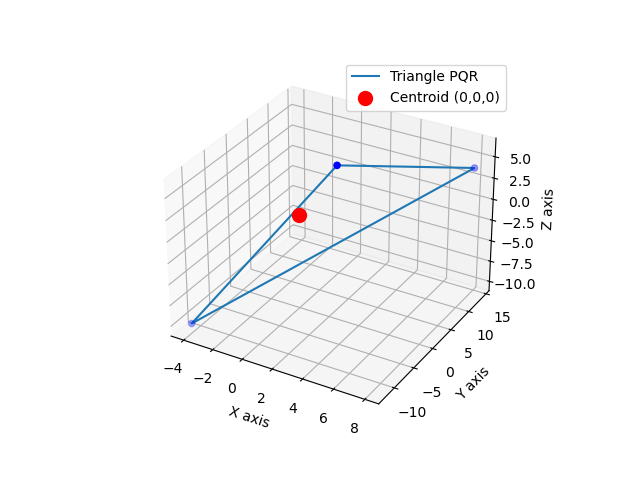
\includegraphics[width=0.7\linewidth]{figs/Figure_1.png}
   \caption{plot for triangle}
   \label{plot}
\end{figure}
\end{document}
